% Drawing 57/16-1 -- folder 57, batch 16, archive page 309 (PDF page 310).
% Transcription: deux droites qui se croisent, marquées $p$
% Kind: two crossing lines marked p. Method 2 (schematic redraw from the facsimile). Status: ok.
% Notes: Two long, nearly horizontal lines crossing (with a third stroke along one of them), and to their right a brace and p.
% Coordinates: 1 unit = 1 mm = 1/100 of the crop width (bbox in page fractions: [0.77, 0.49, 0.9, 0.53]).
% Redrawn by Claude (claude-opus-5-5), issue #73, 2026-11-07; not checked by a human; not compiled (no TeX in the session).
% Rights: reproduces part of the work -- behind RENDER_TRANSCRIPTS, never published by itself.
\documentclass[tikz,border=3pt]{standalone}
\usepackage{amsmath,amssymb}
\usetikzlibrary{patterns,arrows.meta}
\tikzset{pencil/.style={black!45}, struck/.style={black!35}, mark/.style={circle,draw,inner sep=1.3pt}, pt/.style={circle,fill,inner sep=0.9pt}, opt/.style={circle,draw,fill=white,inner sep=1.1pt}}
\begin{document}
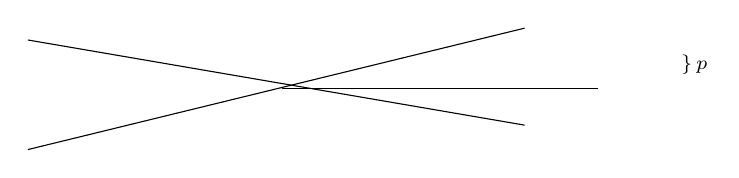
\begin{tikzpicture}[x=1mm,y=1mm,line cap=round,line join=round,font=\scriptsize]
\draw (26.2,-18.2) -- (89.2,-29);
\draw (26.2,-32.1) -- (89.2,-16.7);
\draw (58.5,-24.4) -- (98.5,-24.4);
\node[inner sep=1pt] at (110.8,-21.3) {\scriptsize $\}\,p$};
\end{tikzpicture}
\end{document}
